\documentclass[a4paper,12pt]{report}
\usepackage[left=2.5cm, right=2.5cm, top=3cm, bottom=3cm]{geometry}
\usepackage[T1]{fontenc}
\usepackage{graphicx} % Required for inserting images
\usepackage{hyperref}
\usepackage{listings}
\usepackage{amsmath}
\usepackage[table]{xcolor}
\usepackage{subcaption}

\title{GPU computing}
\author{Simone Petta}
\date{A.A. 2024/2025}

\lstdefinestyle{mystyle}{
    language=C,            % Linguaggio predefinito
    backgroundcolor=\color{gray!10}, % Sfondo leggermente grigio
    basicstyle=\ttfamily\footnotesize, % Font monospace piccolo
    keywordstyle=\color{blue},   % Parole chiave in blu
    stringstyle=\color{red},     % Stringhe in rosso
    commentstyle=\color{green!50!black}, % Commenti in verde scuro
    numberstyle=\tiny\color{gray}, % Numeri di riga in grigio piccolo
    numbers=left,                % Numerazione di riga a sinistra
    stepnumber=1,                 % Numerazione per ogni riga
    showspaces=false,             % Non mostrare spazi
    showstringspaces=false,       % Non mostrare spazi nelle stringhe
    frame=single,                 % Bordo intorno al codice
    tabsize=4,                    % Dimensione del tab
    breaklines=true,              % Abilita il ritorno a capo automatico
    breakatwhitespace=true,       % Va a capo solo sugli spazi
    captionpos=b                  % Posizione della didascalia (b = bottom)
}

\lstset{style=mystyle}
\begin{document}

\maketitle
\tableofcontents

\chapter{Introduzione}
L'obiettivo del corso e' di affrontare il problema del high performance computing.
Affronteremo anche il tema delle GPU e del loro utilizzo nel calcolo ad alte prestazioni. Inoltre useremo il framework CUDA per sviluppare applicazioni parallele utilizzando il linguaggio CUDA-c che e' un estensione del linguaggio c.
Introdurremo anche alcune librerie di python, andando a focalizzarci su elementi a basso livello.

Il parallel computing e' la necessita' di accellerare le computazioni avvalendosi di un numero molteplice di processori. Quando ho un processo di grande dimensioni devo essere in grado di dividere il processo in parti e assegnarlo a vari processi. E' fondamentale la progettazione del problema per spezzettarlo in problemi autonomi.

La CPU ha degli aspetti critici, sono decenni che non vediamo crescere il clock (quante operazioni puo' fare al secondo) si e' andati incontro a misure fisiche che non possono essere superate, come la potenza dissipata.
Una naturale estensione e' stata aumentare il numero di core, da multi core a many many core dando vita a device diversi, le GPU, che riscono a mantenere la legge di Moore e a fare si che a costi bassi una workstation diventi una macchina ad alte prestazioni. Bisogna dare credito a Nvidia che ha creato le general purpose GPU, che sono delle GPU che possono essere utilizzate per calcoli generali e non solo per il rendering grafico.

Il parallel computing e' indipendenza, comunicazione e scalabilita' dei processi.

Le motivazioni che portano all'utilizzo della GPU, un esempio e' la riflessione, rifrazone e ombra, la cosa che si fa e' avere un calcolo semplice che si fa per ogni pixel, quindi calcoli semplici ripetuti un numero esorbitante di volte.
Vengono anche usate per il deeplearning. Perche' le CNN sono di interesse per la GPU? fanno un'operazione basilare da ripetere un numero esorbitante di volte, fanno la convoluzione, prendono un immagine ed un kernel e scandiscono l'immagine sottostante estraendone matrici della dimensione del kernel e fare la somma.
Un altro esempio e' il calcolo matriciale, vengono fatti due prodotti interni tra i vettori riga e colonna delle matrici, questo puo' essere parallelizzato pensando che gruppi di thread distinti possono occuparsi di ogni entry, fare questa cosa in sincrono costerebbe $o(n^3)$.

\section{GP-GPU}
In sistemi eterogenei, le GPU possono essere utilizzate insieme alle CPU per ottenere prestazioni superiori. La chiave per sfruttare al meglio queste architetture eterogenee e' la suddivisione del lavoro tra le diverse unità di elaborazione, in modo che ogni tipo di processore possa occuparsi delle operazioni per cui e' piu' adatto. E' importante notare che questa architettura e' di tipo master-slave, dove la CPU funge da master e le GPU da slave.
Una funzione gpu e' scritta per sfruttare il parallelismo e CUDA ci permette di pensare il sequenziale nonostante poi i calcoli vengano eseguiti in parallelo, l'obiettivo e' aumentare la potenza di calcolo.

\section{Architetture eterogenee}
C'e' la GPU e la CPU, la cpu ha un numero di core. C'e' un bus di ci per la comunicazione tra CPU e GPU.

Quando si crea codice per queste architetture ci si trova con un eseguibile con blocchi di codice che devono essere eseguiti dalla CPU e blocchi dalla GPU.

Le due parti sono destinate a compiti diversi, se i dati sono piccoli e il parellelismo e' basso siamo nel dominio della CPU ed e' quasi inutile fare il parallelismo con la GPU (solo l'overhead del setup iniziale costa di piu') viceversa se i dati sono grandi e il parallelismo e' alto, allora ha senso utilizzare la GPU.

\subsection{Parallelismo delle istruzioni}
Il parallelismo delle istruzioni e' importante (meno di quello dei dati), nel momento in cui il problema puo' essere suddiviso in diverse istruzioni queste vengono eseguite in parallelo. Ci vuole una dotazione hardware adeguata per gestire questo tipo di parallelismo, come ad esempio un numero sufficiente di unità di esecuzione e una gestione della comunicazione tra processi.

\subsection{Parallelismo dei dati}
Noi lavoreremo in una logica sequenziale ma si estende ad una grossa mole di dati. In questo caso, il parallelismo dei dati diventa cruciale, poiché consente di elaborare simultaneamente grandi volumi di informazioni. Utilizzando tecniche di parallelizzazione, possiamo suddividere i dati in blocchi più piccoli e distribuirli su più unità di elaborazione, massimizzando così l'efficienza e riducendo i tempi di calcolo.

\section{Parallelismo di task}
Il fatto di poter avere gruppi di operazioni distinti, ci porta ad un problema non banale di identificazioni di task indipendenti dall'altri, spesso ci si avvale di strumenti come i grafi. Due task sono indipendenti se le operazioni che li compongono non sono dipendenti tra di loro. Questo problema in termini piu' formali e' di colorazione del grado, ogni colore individua un gruppo di nodi indipendnti tra di loro.
Non e' un problema banale, perche' e' irrisolvibile NP-hard, quindi ci si accontenta di soluzioni approssimative.

\section{Tassonomia di Flynn}
Si evidenzia i modelli \textbf{SISD} single instruction single data dove non c'e' nessun parallelismo e le operazioni vengono eseguite sequenzialmente.
In contrapposizione abbiamo il \textbf{SIMD} (single instruction multiple data) dove abbiamo un'istruzione che viene eseguita su piu' dati, sono spesso dotate di librerie e hardware consistente che possono svolgere operazioni parallele, in questo caso c'e' l'accesso ad una memoria globale.
\textbf{MISD} (multiple instruction single data) e' un modello in cui piu' istruzioni vengono eseguite su un singolo dato, mentre il \textbf{MIMD} (multiple instruction multiple data) consente l'esecuzione di piu' istruzioni su piu' dati, rappresentando il massimo livello di parallelismo.

Il modello \textbf{SIMT} e' interessante e viene introdotto da CUDA, qui ci sono tanti thread che svolgono tante operazioni su thread distinti, deve esserci un sistema book treading. C'e' un evoluzione del modello SIMD perche' lo cambia con il modello multithreading, decade il vincolo della singola istruzione, questo e' dato dalla presenza di branch nel codice. Questo modello e' molto utile perche' ci permette di pensare in modo sequenziale anche se complica un po' l'architettura perche' bisogna fare comunicare i thread. Questo e' il modello implementato dai processori GPU.

\begin{figure}
    \centering
    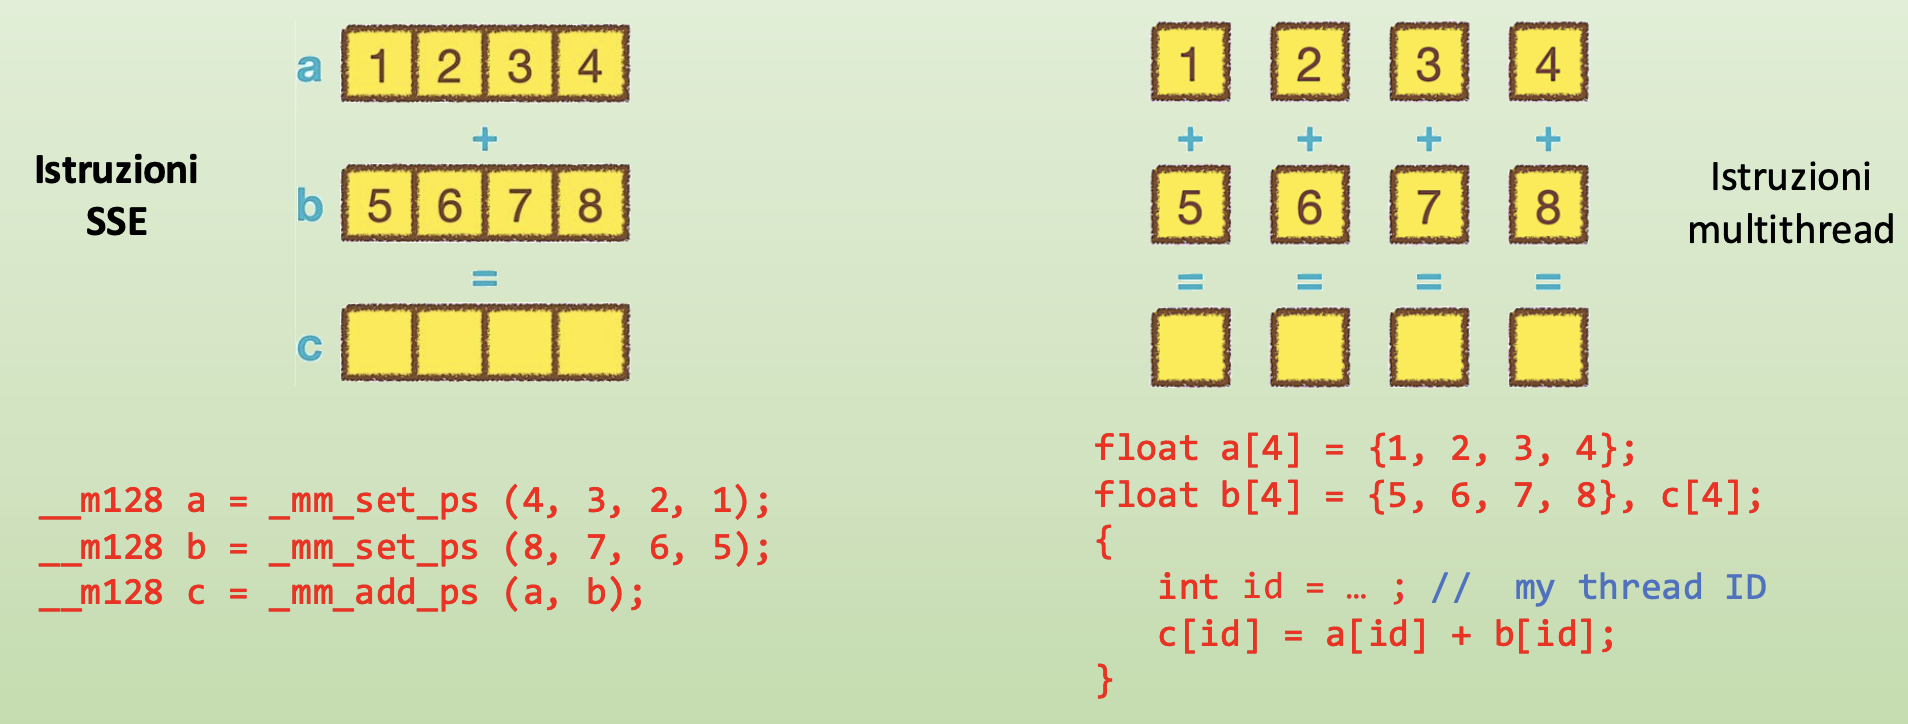
\includegraphics[width=0.8\textwidth]{images/simtvssimd.png}
    \caption{Confronto tra SIMT e SIMD}
\end{figure}

Nel simt si fissano gli operandi, mentre nel simd no.

\section{GPU Nvidia}
CUDA e' una libreria che permette di fare applicazioni sulle GPU

Ogni scheda e' composta da streaming multi processor, ogni streaming contiene dei core che costituiscono l'architettura della scheda, ci sono gli elementi di memoria shared e global.

\subsection{Cuda core}
Un core ha una logica di processazione vettoriale, piu' dati insieme che possono essere caratterizzati da diverse unita' di calcolo (floating point).

\subsection{CUDA}
E' la piattaforma che ci permette di dare luogo ad un modello di programmazione per le schede Nvidia.
Guardando a CUDA nello specifico per progettare delle applicazioni accellerate per le GPU useremo delle libreria gia' accellerate per GPU (come il compilatore).

Ci sono due famiglie di api:
\begin{itemize}
    \item CUDA Runtime
    \item CUDA Driver: sono a basso livello e sono piu' difficili da utilizzare perche' non astraggono determinate cose
\end{itemize}

\subsubsection{Programma CUDA}
Un programma cuda e' composto da due parti:
\begin{itemize}
    \item codice host eseguito su CPU
    \item codice device eseguito su GPU
\end{itemize}

Il compilatore separa il codice host dal codice device in fase di compilazione, generando un file eseguibile che contiene entrambe le parti.

\subsection{Hello world in cuda}

Per scrivere programmi cuda va modificata la sintassi del c, si scrivono delle funzioni che sono destinate al kernel cuda:
\begin{lstlisting}
    __global__ void hello_world() {
        printf("Hello, World from GPU!\n");
    }
\end{lstlisting}

Per invocarla va utilizzata questa sintassi in cui specifichiamo il numero di blocchi e il numero di thread per ogni blocco:
\begin{lstlisting}
    hello_world<<<num_blocks, threads_per_block>>>();
\end{lstlisting}

Il risultato finale e':
\begin{lstlisting}
    __global__ void hello_world() {
        printf("Hello, World from GPU!\n");
    }

    int main(void) {
        hello_world<<<1, 10>>>();
        cudaDeviceReset();
        return 0;
    }
\end{lstlisting}

In questa funzione stamperemo 10 volte "Hello, World from GPU!".

La funzione cudaDeviceReset serve a ripristinare lo stato del dispositivo GPU. Viene utilizzata per liberare le risorse allocate sulla GPU e riportare il dispositivo a uno stato pulito. È buona norma chiamare questa funzione alla fine di un programma CUDA per garantire che tutte le risorse siano correttamente rilasciate.

\chapter{Modello di programmazione CUDA}
\section{Modelli per sistemi paralleli}
E' qualcosa di complesso che richiede una parte HW e software, bisogna necessariamente fare delle astrazioni perche' non ci potremo occupare di tutti i dettagli.
Abbiamo questa astrazione:
\begin{itemize}
    \item Livello macchina: assembly
    \item Modello architetturale: SIMD o MIMD, si prevedono anche processi in cui ci sono tante unita' di calcolo che interagiscono tra di loro, gestione multi processi e multi thread
    \item Modello computazionale: e' un modello formale che consente di descrivere la macchina astraendo dai modello sottostanti ed e' fondamentale per la creazione degli algoritmi. Processore, memoria, scambio dati con un BUS. E' inerentemente sequenziale ma e' utile per creare l'algoritmo data la size dei dati. Nell'ambito del parallelismo passiamo dal modello RAM al PRAM (modello RAM per architetture parallele)
    \item Modello di programmazione parallela: e' il modo con cui gestiamo il sistema di calcolo parallelo esprimendo algoritmi con un linguaggio che espone il prallelismo dell'architettura sottostante per essere eseuito da un linguaggio che ha in se elementi che permettono di usare il parallalismo. Vi sono aspetti di comunicazione per gestire il multi threading, si affronta quindi la suddivisione del compito in processi e thread. Fino ad arrivare a problemi legati all'uso o della gestione di spazi di indirizzamento condivisi.
\end{itemize}

\subsection{SIMD}
Si parla di unita' molteplici che lavorano sui dati, laddove i dati permettono di sviluppare meccanismi paralleli. E' un mondo vasto che si puo' vedere anche nelle architetture comuni dove si ha la divisione di computazione in diverse ALU specializzate, una che lavora su un singolo registro ed una che lavora vettorialmente ed e' quindi in grado di lavorare su piu' dati contemporaneamente. Nelle GPU parleremo di thread che lavorano simultaneamente in modalita' SIMD.

\subsection{MIMD}
E' un'altro dei modelli molto diffusi paralleli in cui si hanno le istruzioni di tanti dati simultaneamente che vengono eseguite da un numero di processori veramente grandi.

\subsection{PRAM}
Il modello PRAM e' il modello di calcolo parallelo piu' semplice, in questo caso abbiamo una memoria condivisa, i processori lavorano in maniera SIMD ovvero fanno la stessa istruzione, esistono anche processori inattivi.
Ci da quanti passi ci servono per risolvere l'algoritmo parallelo, anche in questo caso potremmo fare studio di complessita' per risolvere il problema parallelo.

\subsection{Parallelizzazione di algoritmi}
Quando vorremo vedere la complessita' computazionale degli algoritmi dovremo fare delle astrazioni ed usare qualcosa simile al PRAM.
Nella pratica dovremo vedere come dividere la computazione in parallelo per capire come le varie parti vengano attribuite ai vari thread, tendenzialmente la partizione logica dei task la faremo noi, la parte dello scheduling se ne occupa il sistema ma e' bene conoscela perche' ad esempio in CUDA i processi di scheduling sono fortemente condizionanti dalla potenza del sistema e dovremo adeguare gli algoritmi sulla base dei meccanismi di scheduling. Quello che vorremo ottenere e' una massima occupancy delle unita' di calcolo.

\section{CPU multi-core e programmazione multi-threading}
Un programma in esecuzione e' un processo che viene allocato nel OS e ha una serie di risorse che ha, convive con altri processi nel sistema ed e' una cosa abbastanza pesante, mentre i thread che compongono un processo sono dei sotto-processi ma piu' leggeri. Un processo in genere consiste di tanti thread. In genere vengono creati da delle operazioni di sistema come le fork in UNIX e vengono terminati dall'OS.
I processi hanno il loro contesto e vengono eseguit sequenzialmente secondo un flusso, anche i thread eseguono le cose sequenzialmente ma essendo molteplici possono essere parallali.
Il thread e' un singolo flusso di istruzione che si trova in un processo che lo scheduler si occupa di eseguire concorrentemente ad altri threads.

\subsection{Thread}
Ha un ciclo di vita, viene generato e viene ucciso, il processo chiude quando tutti i thread hanno terminato la loro esecuzione:
\begin{itemize}
    \item New: viene generato, chi lo ha generato sa chi e' 
    \item Executable: il thread e' pronto per essere eseguito quando ha tutte le risorse necessarie
    \item Running: il thread sta attualmente eseguendo le sue istruzioni
    \item Waiting: il thread sta aspettando che una risorsa diventi disponibile
    \item Finished: il thread ha completato la sua esecuzione e viene rimosso
\end{itemize}

I vantaggi sono:
\begin{itemize}
    \item Si possono avere tanti flussi di esecuzioni che possono avvantaggiarsi di sistemi multi-core
    \item Visibilita' dei dati globale
    \item Semplicita' di gestione eventi asincroni come l'io 
    \item Velocita' di context switching
\end{itemize}

Le difficolta' sono la concorrenza e il problema di avere uno spazio privato.

\section{Programmazione multi-core}
Noi vedremo la programmazione multi-thread su architetture multi-core. L'applicazione deve essere progettata considerando diversi fattori del sistema di calcolo parallali multi-core (e many core come le GPU), bisogna trovare di task, bilanciarli, suddividere i dati sui vari task (il problema e i dati lo devono consentire) e farlo in modo che tutti i task possano lavorare su queste porzioni di dati indipendentemente. Ci sono quindi tanti aspetti da tenere in considerazione sulla dipendenza e indipendenza dei dati. Test e debugging sono anchessi importanti quando si sviluppano gli algoritmi in ambito parallelo perche' ci sono tanti flussi di esecuzione.

\section{Flip di un immagine}
Vediamo come applicare la programmazione multi-thread per flippare un immagine, che e' molto parallelizzabile, vogliamo generare una nuova immagine partendo da quella data.

Useremo il formato bitmap in cui ogni riga dell'immagine ha una lungezza n byte multipla di 4, ogni bit e' RGB e c'e' anche un header con dei metadati

\section{Programmazione CUDA}
\begin{itemize}
    \item I dati stanno su host
    \item allocare spazio su GPU
    \item copiare i dati da host a GPU
    \item allocare memoria per l'output
    \item lanciare il kernel che elabora dati in ingresso e li mette in output, mette una copia su memoria condivisa
    \item cancellare le memorie allocate
\end{itemize}

\subsection{Organizzazione dei thread}
Cuda presenta una gerarchia astratta di thread che si distribuisce su due livelli:
\begin{itemize}
    \item grid: una griglia ordinata di blocchi
    \item block: un insieme di thread che possono cooperare tra loro
\end{itemize}
Questi possono avere dimensioni 1D, 2D o 3D. Tutto questo fa 9 combinazioni tra grid e block.
Ci sono delle limitazioni, un blocco puo' contenere al massimo 1024 thread.

Il blocco di thread e' molto importante, dal punto di vista semantico ha un significato importante, possono cooperare tra loro tramite:
\begin{itemize}
    \item sincronizzazione: cooperare per uno stesso compito avvantaggiandosi da operazioni fatte da altri thread
    \item comunicazione tramite la shared memory: e' una memoria cache che quindi ha tempi di accesso di molto ridotti
\end{itemize}

I thread vengono identificati univocamente tramite l'id di blocco e l'id di thread. blockIdx e threadIdx sono specificati in variabili globali, un kernel a runtime ha accesso a queste informazioni che vengono assegnate dinamicamente, hanno tre valori x, y, z di tipo uint32.
Abbiamo accesso alle dimensioni della griglia e del blocco tramite le variabili blockDim e gridDim, che sono anchessi di tipo uint32. Anche in questo caso abbiamo tre componenti x, y, z.

L'indice univoco del thread nei blocchi si calcola differentemente rispetto alle dimensioni del blocco:

\subsection{Lancio di un kernel CUDA}
Quando prendo una funzione e la lancio con un kernel significa che prendo quella funzione e la lancio sulla GPU, i parametri di configurazione di esecuzione sono fatti in questo modo:
\begin{lstlisting}
    kernel<<<gridDim, blockDim>>>(args...);
\end{lstlisting}
Il primo valore \texttt{gridDim} specifica la dimensione della griglia di blocchi, mentre il secondo valore \texttt{blockDim} specifica la dimensione di ciascun blocco di thread. Gli argomenti \texttt{args...} rappresentano i parametri da passare al kernel.

\subsection{Kernel concorrenti}
Potrebbe verificarsi che numerosi kernel vengano lanciati sullo stesso host (dallo stesso processo o da processi diversi), potrei trovarmi nella situazione in cui ho diversi blocchi concorrenti sullo stesso device.

Esiste l'api cudaDeviceSynchronize che permette di sincronizzare l'esecuzione dei kernel, significa che la cpu si sincronizza con tutti i kernel, praticamente il lancio del kernel diventa bloccante.

\subsection{Restrizioni del kernel}
\begin{itemize}
    \item Accede alla memoria globale
    \item Restituisce void
    \item non supporta numero variabile di argomenti, devono essere specificati
    \item non supporta le variabili statiche
    \item ha un comportamento asincrono rispetto al chiamante
\end{itemize}

\subsection{Memoria}
E' praticamente una trasposizione 1 a 1 della memoria in C, le funzioni servono per allocare memoria sul device in global memory (ricordasi che i thread accedono tutti alla global memory):
\begin{itemize}
    \item cudaMalloc: alloca memoria sul device
    \item cudaFree: dealloca memoria sul device
    \item cudaMemcpy: copia dati tra host e device
    \item cudaMemset: imposta un valore nella memoria del device
\end{itemize}
Il trasferimento e l'allocazione di memoria sono operazioni sincrone, l'host si ferma in attesa del completamento di queste operazioni.

cudaMalloc ritorna un doppio puntatore, che e' quello che viene passato ai kernel per puntare correttamente allo spazio di indirizzamento del device (memoria globale), la size e' in byte, il puntatore e' di tipo void\*:
\begin{lstlisting}
    cudaError_t cudaMalloc(void** devPtr, size_t size);
\end{lstlisting}

restituisce un codice di errore. La cudaFree e' quella che libera la memoria.

I puntatori su host e device sono diversi, non e' possibile fare assegnamenti tra uno e l'altro invece bisogna usare la cudaMemcpy.


\chapter{Architetture delle GPU}
\section{Loop Unrolling}
L'idea e' di ottimizzare i loop ripetendo le istruzioni nel corpo del loop. Invece di eseguire un'iterazione alla volta, il compilatore o il programmatore espande il loop per eseguire più iterazioni in un singolo passaggio. Questo riduce l'overhead del controllo del loop e può migliorare l'uso della pipeline della CPU o della GPU.
Come esempio vediamo il for della parallel reduction vista in precedenza:
\begin{lstlisting}
    for (int stride = blockDim.x / 2; stride > 0; stride /= 2) {
        if (threadIdx.x < stride) {
            thisBlock[threadIdx.x] += thisBlock[threadIdx.x + stride];
        }
        __syncthreads();
    }
\end{lstlisting}

Per farlo e' possibile aggiungere un descrittore volatile che implica che ogni volta che l'istruzione viene eseguita va direttamente alla shared memory, evitando ottimizzazioni indesiderate da parte del compilatore passando per la cache:
\begin{lstlisting}
    if (tid < 32) {
        volatile int *vmem = thisBlock;
        vmem[tid] += vmem[tid + 32];
        vmem[tid] += vmem[tid + 16];
        vmem[tid] += vmem[tid + 8];
        vmem[tid] += vmem[tid + 4];
        vmem[tid] += vmem[tid + 2];
        vmem[tid] += vmem[tid + 1];
    }
\end{lstlisting}
32 non e' un numero casuale ma stiamo facendo l'unrolling a livello di warp:
%immagine uso dei thread del warp

\subsection{Block unrolling}
Possiamo estendere l'idea di loop unrolling anche a livello di block. In questo caso, invece di unrollare le operazioni all'interno di un singolo warp, possiamo unrollare le operazioni su più thread all'interno di un block. Questo approccio può portare a un utilizzo più efficiente delle risorse della GPU e a una riduzione del numero di sincronizzazioni necessarie.
%immagine block unrolling

\section{Architetture delle GPU}
Il PCI Express sono i bus che permettono di unire CPU e GPU ed e' normalmente il collo di bottiglia del sistema. Ci sono dei controller da entrambe le parti che permettono di parlare con il BUS, all'interno di CPU e GPU ci sono bus per comunicazione interna molto piu' veloci.

Il PCI Express BUS parla con dei controller che a loro volta si interfacciano con i livello di cache piu' basso dell'architettura.

\subsection{Compute Capability}
E' il termine usato per descrivere la versione hw degli acceleratori GPU che appartengono alle famiglie di dispositivi e che hanno una data architettura interna. E' un parametro che va passato al comiplatore, dobbiamo tenere in considerazione questi cambiamenti generazionali delle GPU per scrivere degli algoritmi efficienti per l'architettura che abbiamo a disposizione.
Non c'e' grande compatibilita' tra versioni.

\subsection{Architettura interna GPU}
Ci sono i vari straming multi processors che comunicano usando una shared memory che e' una memoria cache, poi ci sono i vari bus e controllori che parlano con la CPU.
%immagine

\subsubsection{Host interface}
E' un controller interno alla GPU che si interfaccia verso bus PCie. Consente alla GPU di trasferire dati da e per la CPU. Ha due tipi di memorie cache: una L1 interna al sm e una L2 condivisa tra SM. Ogni cache l1 e' parallela e combina attivita' con le unita' load/store. Un memory controller dedicato trasporta dati dentro e fuori dalla GDDR5 global memory.

\subsubsection{Giga-thread scheduler}
Si occupa di assegnare ai vari SM disponibili ti blocchi del kernel con una politica di round robin. 
L'assegnamento di blocchi a SM e' un attivita' veloce, l'esecuzione molto piu' lenta.
La variabili gridDim, blockIdx e blockDim sono pasate dal giga thread scheduler ad ogni core della GPU che eseguira' il corrispondente blocco.

\subsection{Scheduler di warp}
Ogni blocco e' assegnato a un SM. Ogni SM contiene 2 warp scheduler e 2 instruction dispatch unit. I due scheduler selezionano 2 warp da eseguire in parallelo e distribuiscono un'istruzione a ognuno dei 16 core o alle 16 unita' o alle 4 fpu. L'archittura fermi puo' trattare simultaneamente 8 blocchi = 48 warp per SM per un totale di 1536 thread alla volta residenti su un singolo SM.

\subsection{Fermi: kernel e memoria}
La memoria e' fissa e' puo' essere divisa in\dots

\subsection{Transparent scalability}
E' la capacita' di eseguire lo stesso codice applicativo su diverse architetture, numero variabile di compute core e di SM.

\subsection{Parallelizzazione dinamica}
Potremmo voler lanciare un kern da un kernel, il kernel padre puo' consumare l'output prodotto dal figlio tutto senza la CPU:
\begin{lstlisting}
    __global__ void kernel_figlio() {
        // Codice del kernel figlio
    }

    __global__ void kernel_padre() {
        // Codice del kernel padre
        kernel_figlio<<<1, 1>>>();
    }
\end{lstlisting}

\subsubsection{Bilanciare il lavoro}
Se mi accorgo che un blocco di dati e' molto grande e richiede tanto tempo potrei dividere questo blocco in altri blocchi e dividere il lavoro con altri thread. Questo e' utile per evitare che un singolo blocco di dati rallenti l'intero processo di calcolo.

\chapter{Memorie}
Esiste una gerarchia di memoria, partono da memorie molto veloci come i registri, le cache arriviamo poi alla main memory e alla disk memory, sempre piu' lente e sempre piu' grandi.

Ci sono i principi di localita' e gerarchia di memorie. Il principio di localita' spaziale afferma che i programmi tendono ad accedere a una porzione ristretta di memoria in un dato momento, se accedo ad i e' molto probabile che acceda ad un indirizzo li' vicino (delta i), il che rende vantaggioso mantenere i dati frequentemente utilizzati nelle memorie piu' veloci. La gerarchia di memorie sfrutta questo principio organizzando le memorie in livelli, con memorie piu' veloci e costose in alto e memorie piu' lente e economiche in basso.
Mentre la localita' temporale si riferisce alla tendenza ad eseguire la stessa istruzione piu' volte in un breve intervallo di tempo.

Il modello di memoria CUDA, abbiamo visto che esistono delle memorie programmabili che hanno pattern di accesso utilizzabili con le API di sistema e devono essere gestite direttamente, devono essere gestite in maniera diversa per la lettura e la scrittura. Poi ci sono delle memorie non programmabili, le cache L1 e L2.

\section{Registri}
Sono le memorie piu' veloci e piu' piccole. Sono ripartiti tra i warp attivi (assegnati ad ogni thread). Le variabili locali sono quelle che vengono assegante ai registri senza che sia specificato nessuno dei qualificatori generalmente risiede in un registro.
Meno registri usa il kernel, piu' blocchi di thread e' probabile che risiedano sul multiprocessore, quindi meno ne usiamo meglio e'.

\section{Local Memory}
E' una memoria lenta come la global memory. E' una memoria locale ai thread ed e' usata per contenere le variabili automatiche (grandi) non contenute nei registri:
\begin{itemize}
    \item Array locali i cui indici non possono essere determinati a compile-trasferimento
    \item Strutture locali grandi che consumano troppo spazio registro
    \item Ogni variabile che non puo' essere allocata nei registri a causa numero limitato (register spilling)
\end{itemize}
Risiede nella device memory, pertanto gli accessi hanno stessa latenza e ampiezza di banda della global memory e sono soggetti anche agli stessi vincoli di di coalescenza.
Il compilatore nvcc si preoccupa della sua allocazione e non e' controllata dal programmatore.

\section{Constant Memory}
Risiede in device memory ed ha una cache dedicata in ogni SM. E' ideale per ospitare dati a cui si accede in modo uniforme e in sola lettura. 
Una variabile dichiarata come \texttt{\_\_constant\_\_} viene dichiarata con scope globale, ad di fuori di qualsiasi kernel. 
L'utilizzo migliore come dice il nome e' allocarci dati che devono essere distribuiti tra tanti kernel.

\begin{lstlisting}
    cudaError_t cudaMemcpyToSymbol(const void *symbol, const void *src, size_t count);
\end{lstlisting}

E' pari a 64KB per tutte le compute capability.

\section{Texture Memory}
E' una memoria in sola lettura, dotata di cache e risiede in device memory. E' particolarmente utile perche' include un supporto hw efficiente per filtraggio o interpolazione floating-point nel processo di lettura dei dati. E' ottimizzata per la localita' spaziale 2D, quindi dati espressi sotto forma di matrici.
I thread di un warp che usano la texture memory per accedere a dati 2D hanno migliori prestazioni rispetto a quelle standard.

\section{Shared Memory}
E' una memoria programmabile on-chip con un bandwidth molto piu' alto e minor latenza della local o global memory. E' suddivisa in moduli della stessa ampizza, chiamati bank che possono essere acceduti da un thread alla volta.
Abbiamo 32 banchi di memoria che devono essere utilizzati in maniera opportuna per essere acceduti simultaneamente.
Ogni SM ha una quantita' limitata di shared memory che viene ripartita tra i blocchi di thread. 
Bisogna farne un uso parco ancora una volta per non limitare il numero di warp attivi.
Con i blocchi di thread condivide anche lifetime e scope.
E' fondamentale per la comunicazione inter-thread di un blocco, poiche' permette di scambiare dati in modo rapido e con bassa latenza.
L'accesso deve essere sincronizzato per mezzo delle seguente CUDA runtime call:
\begin{lstlisting}
    __syncthreads();
\end{lstlisting}

%metti immagine

\subsection{Organizzazione}
La SMEM dell'arch Fermi sono suddivisi in blocchi da 4 byte (chiamate word) da 32 bit (0 64). Ogni word puo' contenere tipi base (1 int, 1 float, 2 short, 4 char).
la bandwitdth e' di 32 bit ogni 2 cicli di clock.
Nei 32 banchi andiamo ad accedere simultaneamente a 32 word, ed e' l'accesso piu' veloce che possiamo avere:
%immagine organizzazione

\subsection{SMEM runtime}
Viene ripartita tra tutti i blocchi residenti in un SM. Maggiore e' la shared memory richiesta da un kernel, minore e' il numero di blocchi attivi concorrenti. Il contenuto della shared memory ha lo stesso lifetime del blocco cui e' stata assegnata. L'accesso e' per warp: caso migliore 1 transazione x 32 thread, caso peggiore 32 transazioni.

\subsection{Pattern di accesso}
Se un'operazione di load o store eseguita da un warp richiede al piu' un accesso per bank, si puo' effettuare in una sola transizione il traferimento dati dalla shared memory al warp.

%esempio

\begin{itemize}
    \item Caso broadcast: un singolo valore letto da tutti i thread in un warp da un singolo bank
    \item Caso parallelo: un singolo valore letto da un singolo bank. In questo caso le cose vanno bene, per ogni thread accediamo al corrispondente banco di memoria.
    \item Conflitto doppio: tutti i thread di un warp richiedono una word di indice doppio il threadId.x
    \item Nessun conflitto: strutture di 3 word come, ad esempio, le terne di punti nello spazio.
\end{itemize}

\subsection{Conflitto di accesso}
Il bank conflit e' quando diversi indirizzi di shared memory insistono sullo stesso bank. L'hw effettua tante transizioni quante ne sono necessarie per risolvere il conflitto, riducendo le prestazioni.

%esempio

\subsection{Configurazione SMEM / cache L1}
Ogni SM ha 64 Kb di memoria on-chip, la sherd memory e L1 cache condividono questa risorsa HW. 
Cuda fornisce due metodi per configurare la L1 cache e la shared memory:
\begin{lstlisting}
   cudaError_t cudaDeviceSetCacheConfig(cudaFuncCache cacheConfig);
\end{lstlisting}

Dove l'argomento cacheConfig specifica come deve essere ripartita la memoria:
\begin{itemize}
    \item cudaFuncCachePreferNone: no preference
    \item cudaFuncCachePreferShared: prefer shared memory 48KB shared e 16 Kb L1
    \item cudaFuncCachePreferL1: prefer L1 cache
    \item cudaFuncCachePreferEqual: equal preference
\end{itemize}

\subsection{Osservazioni}
Il latency hiding e' sempre una cosa indesiderata, il ritardo che puo' incorrere alla SMEM e all'ottenimento dei dati non e' in generale un problema anche in caso di conflitti di banchi, perche' se si riesce a tenere alto il numero di warp attivi, thread in esecuzione e blocchi letti in esecuzione si ha sempre un sostituto nel momento in cui un warp va in attesa.
Inter-block conflict, non esiste un conflitto tra thread appartenenti a blocchi differenti, il problema sussite solo a livello di warp dello stesso blocco.
Il modo piu' semplice per avere prestazioni elevate e' quello di fare in modo che un warp acceda a word consecutive in memoria shared.
Caching: con lo scheduling efficace le prestazioni anche in presenza di conflitti a livello di SMEM sono di gran lunga migliori se paragonate a quelle in cui il cammino che i dati percorrono passa attraverso la cache L2 o peggio, arriva in global memory.

\subsection{Allocazione statica delle SMEM}
Una variabile in shared memory puo' anche essere dichiarata sia locale a un kernel sia globale in un file sorgente.
E' dichiarata con il qualificatore \texttt{\_\_shared\_\_}.
Puo' essere dichiarata sia staticamente sia dinamicamente.

\subsection{Allocazione dinamica della SMEM}
Se la dimensione non e' nota a tempo di compilazione e' possibile dichiarare una variabile adimensionale con la keyword extern:
\begin{itemize}
    \item Dinamicamente si possono allocare solo array 1D
    \item puo' essere sia internal al kernel sia esterna
\end{itemize}

\subsection{Uso tipico}
\begin{itemize}
    \item Caricare i dati dalla device memory alla shared memory
    \item Sincronizzare i thread del blocco al termine della copia che ognuno effettua sulla shared memory (cosi' che ogni thread possa elaborare dati certi nel prosieguo)
    \item Elabora i dati in shared memory
    \item Sincronizza per essere certi che la shared memory contenga i risultati aggiornati
    \item Scrivi i risultati dalla device memory alla host memory
\end{itemize}

\subsection{Prodotto matriciale con SMEM}
Nella versione senza memoria shared ogni thread e' responsabile del calcolo di un elemento della matrice prodotto. Dobbiamo tenere conto che abbiamo una suddivisione logica dei thread che stanno in un blocco e degli elementi in memoria corrispondenti.
Passi con shared memory:
\begin{itemize}
    \item Occorre caricare in memoria shared i dati relativi ad ogni blocco prima di svolgere le somme e i prodotti
    \item Ogni thread accumula i risultati di ognuno di questi prodotti (scandendo tutti i blocchi) in un registro
    \item Alla fine scrive su global memory
\end{itemize}

Qui l'idea e' di trasferire gli elementi di riga e colonna delle due matrici in shared memory perche' dobbiamo accedere ad ogni elemento tante volte e quindi l'accesso a quella memoria sarebbe piu' veloce.


L'idea e':
\begin{itemize}
    \item Caricare il primo tile 
    \item Effettuare le somme parziali per ogni cella
    \item Riptere per il numero di tile contenuti nelle zone delle matrici da caricare
    \item Scrivere i risultati dalla shared memory alla global memory
\end{itemize}

\subsection{Prodotto convolutivo con SMEM}
La convoluzione e' un prodotto tra due vettori, tendenzialmente un vettore piu' grande ed uno piu' piccolo chiamato kernel o maschera.

Una volta che abbiamo la scrittura matematica l'istanziazione e' con vettori, nell'esempio vediamo il segnale e la maschera, viene evidenziato il segnale centrale perche' e' quello in output della convoluzione:
%metti immagine implementazione
Occorre fare shiftare la maschera con uno stride = 1 e calcolare prodotti e somme.

Da notare che ci sono casi particolari, nell'esempio partiamo dal terzo elemento perche' c'e' corrispondenza reale con la maschera, si potrebbe anche adottare approcci diversi relativamente a dati mancanti.

Questa cosa si estende naturalmente a piu' dimensioni, questo e' l'esempio del 2D:
%esempio immagini 2D

Ha senso pensare all'uso della shared memory perche' alcune celle della matrice di input vengono riutilizzate più volte durante il calcolo della convoluzione (tutte quelle sotto la maschera sicuramente).

Questo e' un problema ideale per il parallel computing:
\begin{itemize}
    \item Determinare la mappa tra thread ed elementi di output
    \item Semplice approccio nei casi 1D e 2D e' organizzare i thread in grid corrispondenti in modo tale che ogni thread calcoli un elemento della matrice di convoluzione 
    \item Problema: non soddisfa per inefficienza negli accessi alla global memory
\end{itemize}

%esempio convoluzione parallela

\subsubsection{Tiling}
Divido i dati in blocchi (ad esempio, 16 elementi in 4 blocchi da 4 thread), ogni thread nel blocco fa un prodotto della convoluzione. Per ridurre l'accesso alla global memory, in cache/memoria condivisa si tengono i dati a cui l'accesso è fatto più frequentemente, ovvero i valori del "blocco di dati" assegnato al block (tutti i thread devono calcolare sullo stesso insieme di dati, o quasi), tenendo conto della dimensione della maschera (serve avere i dati "adiacenti" al blocco, quelli che sbordano (sarebbe molto utile un'immagine, si capirebbe subito)).

I dati da caricare in smem sono più dei thread nel blocco ("alone" che va al di fuori del blocco di dati stesso); in smem carico tutti i possibili dati a cui il blocco deve fare l'accesso. 

Chi carica che dati in memoria? I dati esterni al blocco potrebbero essere anche più del blocco stesso (maschera "grossa"). La soluzione è dare un ordine ai thread e dividere il più equamente possibile i caricamenti in memoria tra i thread del blocco. Si può fare facendo un tiling dei dati da caricare: il blocco viene "ripetuto" sui dati da caricare, secondo un ordine dei thread.


\end{document}